\subsection{Encrypted-Statistics-Service}
\label{sub:encrypted_statistics_service}

\subsubsection*{Funktionsbeschreibung}

\textbf{Akteure}: 
Client (Browser, Angular-Frontend), Server (Axum/Rust-Service). \par
UC5 berechnet statistische Kennzahlen (Summe, Anzahl, Minimum, Maximum, Durchschnitt, Median) über eine Ganzzahlen-Liste, ohne dass der Server die Eingabewerte oder Ergebnisse jemals im Klartext sieht. Alle Berechnungen laufen vollständig auf verschlüsselten Daten.

\textbf{Ablauf eines Requests} (UC5 ist zustandslos — jeder Request ist in sich abgeschlossen):
\begin{figure}[h!]
    \centering
    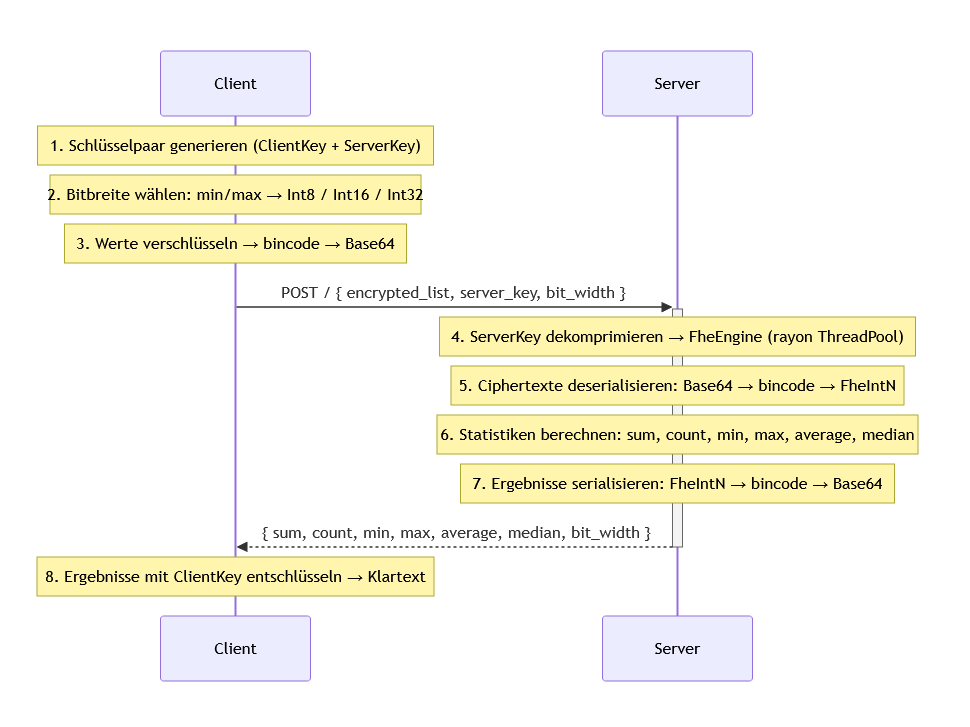
\includegraphics[width=\textwidth]{contents/media/Ablaufsdiagramm_Statistics.png}
\end{figure}

\subsubsection*{OpenAPI-Schnittstelle}

\textbf{POST /}:
Berechnet alle Statistiken für eine verschlüsselte Ganzzahlen-Liste.

\textbf{Request-Schema}:
\begin{lstlisting}
{
  "encrypted_list": [
    "<Base64-String>",
    "..."
  ],
  "server_key": "<Base64-String>",
  "bit_width": 8
}
\end{lstlisting}\par
\begin{tabular}{||l|l|p{9cm}||}
    \hline
    \textbf{Feld} & \textbf{Typ} & \textbf{Beschreibung} \\
    \hline\hline
    \verb|encrypted_list| & \verb|string[]| & Jedes Element: Base64(bincode(FheInt\verb|N|)), wobei N = \verb|bit_width|. Mindestens 1 Element. \\
    \hline
    \verb|server_key| & \verb|string| & Base64(bincode(CompressedServerKey)) - vom Client generiert, enthält kein Geheimnis. \\
    \hline
    \verb|bit_width| & \verb|number| & Muss 8, 16 oder 32 sein. Wird vom Client automatisch aus dem Wertebereich der Eingabe gewählt. \\
    \hline
\end{tabular}

\textbf{Response-Schema (200 OK)}:
\begin{lstlisting}
{
  "sum":       "<Base64-String>",
  "count":     42,
  "min":       "<Base64-String>",
  "max":       "<Base64-String>",
  "average":   "<Base64-String>",
  "median":    "<Base64-String>",
  "bit_width": 8
}
\end{lstlisting}

\begin{tabular}{||l|l|p{9cm}||}
    \hline
    \textbf{Feld} & \textbf{Typ} & \textbf{FHE-Typ (je nach} \verb|bit_width|\textbf{)} \\
    \hline\hline
    \verb|sum| & \verb|string| & Base64(bincode(FheInt16/32/64)) - eine Stufe breiter als Eingabe \\
    \hline
    \verb|count| & \verb|number| & Klartextzahl - dem Server schon aus dem Request bekannt \\
    \hline
    \verb|min| & \verb|string| & Base64(bincode(FheInt8/16/32)) - gleiche Breite wie Eingabe \\
    \hline
    \verb|max| & \verb|string| & Base64(bincode(FheInt8/16/32)) - gleiche Breite wie Eingabe \\
    \hline
    \verb|average| & \verb|string| & Base64(bincode(FheInt16/32/64)) - eine Stufe breiter als Eingabe \\
    \hline
    \verb|median| & \verb|string| & Base64(bincode(FheInt8/16/32)) - gleiche Breite wie Eingabe \\
    \hline
    \verb|bit_width| & \verb|number| & Tatsächlich verwendete Bitbreite: 8, 16 oder 32 \\
    \hline
\end{tabular}

\textbf{Fehlerstatus}:\par
\begin{tabular}{||l|p{9cm}||}
    \hline
    \textbf{Status} & \textbf{Bedeutung} \\
    \hline\hline
    400 Bad Request & Leere Liste, ungültiger Base64, falscher Ciphertext-Typ, ungültige \verb|bit_width| \\
    \hline
    500 Internal Server Error & Serialisierungsfehler beim Zusammenstellen der Response \\
    \hline
\end{tabular}

\textbf{Weitere Endpunkte}:\par
\begin{tabular}{||l|l|p{9cm}||}
    \hline
    \textbf{Endpunkt} & \textbf{Methode} & \textbf{Beschreibung} \\
    \hline\hline
    \verb|/healthz| & GET & Liveness-Probe (Kubernetes) \\
    \hline
    \verb|/readyz| & GET & Readiness-Probe (Kubernetes) \\
    \hline
    \verb|/version| & GET & Service-Version als JSON \\
    \hline
    \verb|/metrics| & GET & Prometheus-Metriken \\
    \hline
    \verb|/docs| & GET & Swagger UI (OpenAPI-Dokumentation) \\
    \hline
    \verb|/openapi.json| & GET & OpenAPI-Spec als JSON \\
    \hline
\end{tabular}

\subsubsection*{Trust- und Threat-Model}
\textbf{Was am Server bekannt ist}:\par
\begin{tabular}{||p{4cm}|p{4cm}|l|p{4cm}||}
    \hline
    \textbf{Datum} & \textbf{am Server klar} & \makecell{\textbf{am Server}\\\textbf{verschlüsselt}} & \textbf{nur am Client} \\
    \hline\hline
    Eingabewerte (die eigentlichen Zahlen) & \makecell{X} & FheInt8/16/32 & Klartext vor Verschlüsselung \\
    \hline
    Anzahl der Elemente (n) & (Array-Länge im Request) & \makecell{-} & \makecell{-} \\
    \hline
    Wertebereich-Klasse & (über \verb|bit_width|: Int8 $\rightarrow$ Werte in [-128, 127]) & \makecell{-} & \makecell{-} \\
    \hline
    Summe & \makecell{X} & FheInt16/32/64 & nach Entschlüsselung \\
    \hline
    Minimum & \makecell{X} & FheInt8/16/32 & nach Entschlüsselung \\
    \hline
    Maximum & \makecell{X} & FheInt8/16/32 & nach Entschlüsselung \\
    \hline
    Durchschnitt & \makecell{X} & FheInt16/32/64 & nach Entschlüsselung \\
    \hline
    Median & \makecell{X} & FheInt8/16/32 & nach Entschlüsselung \\
    \hline
    ServerKey & (aus Request) & \makecell{-} & \makecell{-} \\
    \hline
    ClientKey & \makecell{X} & - & verlässt den Browser nie \\
    \hline
    Anfragezeitpunkt & (HTTP-Timestamp) & \makecell{-} & \makecell{-} \\
    \hline
    Payload-Größe & (HTTP-Header) & \makecell{-} & \makecell{-} \\
    \hline
\end{tabular}

\textbf{Beobachtbare Metadaten und möglicher Missbrauch}:
\begin{itemize}
    \item Anzahl n ist vollständig sichtbar. Ein Angreifer kann daraus schließen, wie viele Werte analysiert werden (z.B. \enquote{der Client hat genau 3 Werte geschickt} $\rightarrow$ möglicherweise 3 Messwerte eines Sensors).
    \item \verb|bit_width| verrät die Größenordnung: \verb|bit_width=8| bedeutet, alle Werte liegen in [-128, 127]. Das schränkt den möglichen Werteraum erheblich ein - bei kleinen Eingabelisten und bekanntem Kontext könnten Werte erraten werden.
    \item Request-Timing ist bei bekannten n-Werten korrelierbar. Die Berechnungsdauer hängt von n und \verb|bit_width| ab, nicht von den konkreten Werten - es gibt kein datenwertabhängiges Timing-Leak.
    \item Payload-Größe ist deterministisch aus n und \verb|bit_width| ableitbar (alle FHE-Ciphertexte haben bei gleichen TFHE-Parametern konstante Größe). Kein zusätzlicher Informationsgewinn.
\end{itemize}

\textbf{Restvertrauen in den Server-Operator}:
Der Server muss die Berechnungen korrekt ausführen. Ein böswilliger Server könnte:
\begin{itemize}
    \item Falsche verschlüsselte Ergebnisse zurückgeben (der Client kann das nicht verifizieren - kein ZKP).
    \item Die Ciphertexte dauerhaft speichern (für einen hypothetischen späteren Kryptangriff).
    \item Den Request einfach ablehnen (Denial of Service).
\end{itemize}

\textbf{Annahmen außerhalb von FHE}:
\begin{itemize}
    \item TLS zwischen Client und Server (kein Mitlesen im Transit).
    \item Das Angular-Frontend und der Browser sind nicht kompromittiert (ClientKey liegt im WASM-Speicher).
    \item TFHE-rs wird als korrekte Blackbox behandelt - keine eigene Kryptanalyse.
    \item Kein Auth-Gateway: jeder kann beliebige Requests an \verb|POST /| schicken.
\end{itemize}

\textbf{Sicherheitsgarantie}:
Der Server kennt die statistischen Kennzahlen der Eingabewerte nicht — er berechnet sie, ohne sie je zu sehen. Bekannt sind ihm nur die Anzahl der Werte und der grobe Wertebereich (über \verb|bit_width|). Keine ZKP-Verifikation der Ciphertexte und keine Client-Authentifizierung — beides ist im Rahmen dieses Use Cases nicht vorgesehen.

\subsubsection*{FHE-Designentscheidungen}

\subsubsection*{Komplexität der eigenen Algorithmen}

\subsubsection*{Performance-Messung}

\subsubsection*{Limitationen}